\documentclass[varwidth=true, border=2pt]{standalone}
\usepackage{tikz}
\usepackage{tkz-euclide}

\begin{document}
\usetkzobj{all}
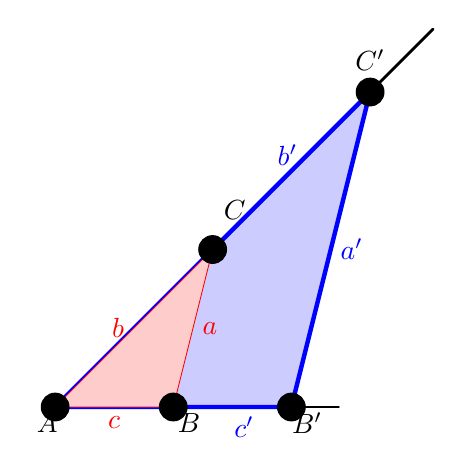
\begin{tikzpicture}
    \tkzSetUpPoint[shape=circle,size=10,color=black,fill=black]
    \tkzSetUpLine[line width=1]
    \tkzDefPoints{0/0/A, 3/0/B', 2/2/C, 4/4/C'}
    \tkzDefLine[parallel=through C](B',C') \tkzGetPoint{Phelper}
    \tkzInterLL(A,B')(C,Phelper) \tkzGetPoint{B}
    \tkzDrawLine[add=0 and 0.2](A,B')
    \tkzDrawLine[add=0 and 0.2](A,C')
    \tkzDrawSegment(B',C')

    \node at ($(A)+(-0.1,-0.2)$)  {$A$};
    \node at ($(B')+(0.2,-0.2)$)  {$B'$};
    \node at ($(C')+(0,0.4)$)  {$C'$};
    \node at ($(B)+(0.2,-0.2)$)  {$B$};
    \node at ($(C)+(0.28,0.5)$)  {$C$};
    \tkzDrawPolygon[ultra thick,color=blue,fill=blue!20](A,B',C')
    \tkzDrawPolygon[line width=0.3pt,color=red,fill=red!20](A,B,C)
    \tkzDrawPoints(A,B',C',B,C)
    \tkzLabelSegment[below,red](A,B){$c$}
    \tkzLabelSegment[left,red](A,C){$b$}
    \tkzLabelSegment[right,red](B,C){$a$}
    \tkzLabelSegment[below,blue,pos=0.8](A,B'){$c'$}
    \tkzLabelSegment[left,blue,pos=0.8](A,C'){$b'$}
    \tkzLabelSegment[right,blue](B',C'){$a'$}
\end{tikzpicture}
\end{document}
